\documentclass[12pt]{article}
\usepackage{fullpage}
\usepackage{times}
\usepackage{graphicx}
\usepackage{natbib}
\bibpunct{(}{)}{,}{a}{}{,}

\bibliographystyle{plainnat}

\setlength{\parindent}{0em}
\setlength{\parskip}{1ex}

\usepackage{squeeze}


\title{Creating a Scalable and Reliable Peer Assessment System for
  Mathematical Proofs}

\author{Randal E Bryant \\ Luis Von Ahn}

\begin{document}

\section*{Project Description}

This research seeks to devise and evaluate mechanisms that will enable
students to get useful and reliable assessments of the proofs they
write in mathematics and computer science classes from their
peers---both students currently enrolled in the class and those who
have taken the course recently and are now serving as graders.  It
also seeks to maximize the educational benefit to the students
performing the assessments, by teaching them how to critically review
and evaluate proofs.  Within the scope of this proposal, the work will
focus on developing and evaluating a system to support the assessment
of proof-based assignments in large classes, with enrollments of 200
or more students.  It will also begin the design of a
system that can support web-scale courses with 10,000 or more
participants.

Our long-term goal is to create educational technology for helping
students learn to write good proofs in large-scale learning
environments.  The resulting technology will also provide a platform
for experimenting with different teaching and assessment strategies
that will enable quantitative evaluation with an unprecedented
degree of scale and granularity.

For {\bf intellectual merit}, this research will study a new realm of
human computation, harnessing the abilities of students with limited
mathematical training to provide reliable and useful assessments of
proofs.  It will devise structured frameworks in which to analyze
proofs, so that assessment can be decomposed into a number of tasks,
each of which can be performed by nonexperts.  Identifying these
structures will also lead to a deeper understanding of how to teach
the writing of proofs.  In addition, it will explore ways to maximize
the learning experience students gain by critically evaluating each
other's proofs.  By supporting web-scale courses, it will create a
platform on which rigorous and large-scale experiments can be
conducted on the effectiveness of different strategies for teaching
students how to write and review mathematical proofs.

As {\bf broader impacts}, this research seeks to enable students in
large classes and in web-scale courses to enhance their learning by
receiving useful feedback on proofs they write.  It will bring to
large numbers of students an educational opportunity that is otherwise
available only in environments consisting of small numbers of students
getting attention from expert mentors.  


\section{Motivation}

Writing clear and concise proofs is a fundamental skill
in mathematics.  Writing a good proof requires the ability to
rigorously decompose an argument into a sequence of steps that lead
from a set of premises to
a desired conclusion.  It also requires the
writer to communicate to the reader enough insight and information to guide them
through the reasoning process at an appropriate level of detail.

Being able to write proofs is also a fundamental requirement in the
education of computer scientists.  Not only does it provide a
mechanism with which they can formally verify that a program will function
correctly \citep{hoare-cacm69}, it also enables them to analyze the
time and space complexity of an algorithm or program.  Even though few
programmers prove theorems about their programs on a routine basis,
knowing how to do so sharpens their ability to systematically reason
about code as they create it.  It also helps them reason through a
specific execution when they try to debug it, determining both how
they arrived at this point in the program and what changes must be
made to prevent an error from occurring.

Learning how to write good proofs can be very challenging for many
students.  In many ways, it is like learning to write a compelling
essay or to paint a beautiful picture---it requires internalizing a
core set of rules and technical skills, while also learning how to
communicate concepts to others. 
Studies have shown that learning to write proofs requires
considerable practice, with feedback based on both an ideal model of a
correct proof, and the buggy models of possible errors
\citep{anderson-jls95}.  Just as with creative writing or art, the
ideal learning environment for proof writing is one where students get
personal attention by expert mentors \citep{anderson-ijcai85}.

Unfortunately, most undergraduate students get their early training in
mathematics and computer science in large classes, where it is
impractical for the instructor to give each student extensive
individual guidance.  If students are to learn to write proofs
starting at an early point in their mathematical and computer science
education, there must be a system for providing them accurate and
timely assessment of their work even in the context of high enrollment
classes.  Such assessments are essential to help them improve their
abilities (formative) and to give them proper credit for their efforts
(summative.)

As a case in point, we recently revised the undergraduate computer science
curriculum at Carnegie Mellon University so that all majors and many
nonmajors take two introductory programming courses---one on imperative programming
and one on functional programming---that have students writing and
proving preconditions, postconditions, and invariants
\citep{bryant-ugrad10}.  Students also take courses in
discrete mathematics and introductory theoretical computer science
that involve proofs and formal reasoning, all within their first two years.
These courses each have
total annual enrollments of 200--500 students.  We handle our
assessment needs with large teams of undergraduate graders, who are
among our best students, but they still lack extensive experience in
the subject material and in critically evaluating proofs.  Ensuring
reliable, consistent, and uniform grading in such environments has proved
challenging.

Going beyond the need to provide assessments for classes with
enrollments in the hundreds, consider the recent advent of {\em web-scale}
courses, such as Massively Open Online Courses (MOOCs),
 offered to 10,000 or more students for free over the Internet
\citep{carson-am12,lewin-nyt12}.
Although it is easy enough to provide simple
assessments to these students, such as multiple-choice questions, 
there is no feasible way to have students attempt to write proofs and
then get reliable feedback on their efforts.  This shortcoming
seriously reduces the degree to which the participants can gain a deep
understanding of mathematics or the theoretical aspects of computer science.

In computer science terms, we require a system for providing
assessments of proofs that is {\em scalable}, meaning that it can meet
the quantitative and qualitative demands for assessments using the
limited resources available.  We consider scaling at both the
large-class and web-scale levels, but with 
resources limited to: 1) an instructor, 2) a small team of assistants,
who may range in talent from almost novices to near experts, and 3) the
students themselves, who are just learning the material and who have
almost no experience in critically evaluating proofs.

We approach this problem as one of {\em human computation}, using
computer technology to devise systems in which useful work can be done by
harnessing the power of large numbers of nonexperts
\citep{quinn-chi11, vonahn05}.  This requires
the task to be decomposed into smaller units of work, each of which 
can be performed by the available talent pool.  It also requires
mechanisms to generate these units, supply them to the workers, and
then aggregate the results, such that the outcome is valid, even when
some of the workers either inadvertently or maliciously misuse the system.

The potential impact of a scalable system for assessing proofs could
be quite profound.  Being able to handle large enrollment classes
would make it possible to run courses with proof-based assignments at
colleges and universities across the entire U.S., and indeed much of
the world.  Web-scale courses are nearing the point of having 100,000
participants.  Equipping them with the ability to provide high quality
feedback to the students as they learn to write proofs would create an
effective learning environment that is available not just to college
students, but to anyone with the ambition to learn.  Looking further,
we can see that there are many millions of people in the world who
would benefit from an education in mathematics, but they have neither
the resources nor the opportunity to do so.  Only by creating truly
scalable systems can we hope to meet the educational needs of the world.

\section{Existing Work on Peer Assessment}

As background, we consider the work done by others, as well as the
prototype system we have developed.

\subsection{Published work}

The published literature on teaching students how to write good proofs
and how to assess their work is remarkably sparse.  Most published
work focuses on creating a tightly knit group of students working
under the close supervision of an instructor
\citep{cohen-amm82,jones-amm77}, or a small-enrollment, seminar-style
course \citep{reisel-amm82}.  These environments allow students to
discuss and evaluate each other's work, but they cannot be scaled to
larger classes.  Indeed, it seems that most math programs avoid
proof-based assignments with their large-enrollment, introductory
courses.

Important work has been done on the use of computer-based tools for
teaching students to prove mathematical theorems.
These include computerized tutors
for high school geometry \citep{anderson-ijcai85} and introductory formal
logic \citep{scheines-93,scheines-94}.  These tutors incorporate proof checkers
that can evaluate the correctness of the students' proofs and even
provide guidance in how to correct erroneous proof steps.  Such a level
of automation is possible in these two domains, because the proofs are
written at a very low level of detail, explicitly stating the
justification of each inference step in terms of previous steps.
Researchers at Stanford have
developed a computer-based proof environment for use in a variety of
mathematics classes \citep{sommer-jar04}.  It uses symbolic algebra and
automatic theorem proving techniques to try to infer the steps that
are normally omitted in a proof intended for human readers rather than
computerized checkers.  Ultimately, however, it is up to the students
to provide enough guidance so that the program can reliably check the
validity of the proof.  These tools differ from our approach in that
they require students to write proofs that are to be read by
computers, rather than by other humans.  There is a large stylistic
difference between these two forms of proof.  The former is like
writing a program: it must follow a very strict and formal structure,
whereas the latter is more like an essay: it must conform to a logical
structure, but it need not give explicit, low-level details.  There is
presently no automated proof checker that can verify the
proofs written by students in typical college-level
mathematics and computer science courses.

The common approach for grading an assignment for a large
class with multiple graders is for the instructor to generate a {\em
  scoring rubric} giving a detailed description of what components the
solution must contain, how each of these components should be
evaluated, and how points should be assigned
\citep{moskal-pa2000}.  Anyone who has tried devising a
good scoring rubric knows that is a very difficult task.  Covering all of the
possible cases, and having it assign consistent and appropriate scores
requires considerable effort.  Quite commonly, the rubric must be
revised as the grading proceeds, requiring assignments to be
regraded.  Even more work is required to ensure quality control, for
example by spot-checking a large collection of assignments to see if
the rubric was followed properly.
In addition, grading proofs from a rubric still requires a great deal of
sophistication, because the grader must have a complete understanding
of the purported proof, including identifying its flaws.
In our experience, even our 
undergraduate graders require several months of
practice before they become reasonably proficient.  As such, it cannot serve as
the basis for a peer assessment system.

Perhaps the most relevant prior work was done by \citet{zerr-primus11} at the
University of North Dakota
They instituted formal peer evaluation, but
in a way that actually increased the required effort by the
instructor, rather than reducing it.  Even so, it produced some
useful insights into the challenges of peer assessment.  They found
the students were good at identifying correct proofs and then
supplying useful advice on how to improve the presentation.  For
incorrect proofs, however, many of the reviewers failed to even detect
that they were incorrect, and even fewer were able to pinpoint the exact error.

Other computer scientists have created generic, online peer review systems
\citep{gehringer-sigcse05, wolfe-ite04}, but these did not address the
assessment of proofs explicitly, and indeed provided little or no
framework for guiding the assessment process.

\subsection{Our Prototype System}

\begin{figure}
\begin{center}
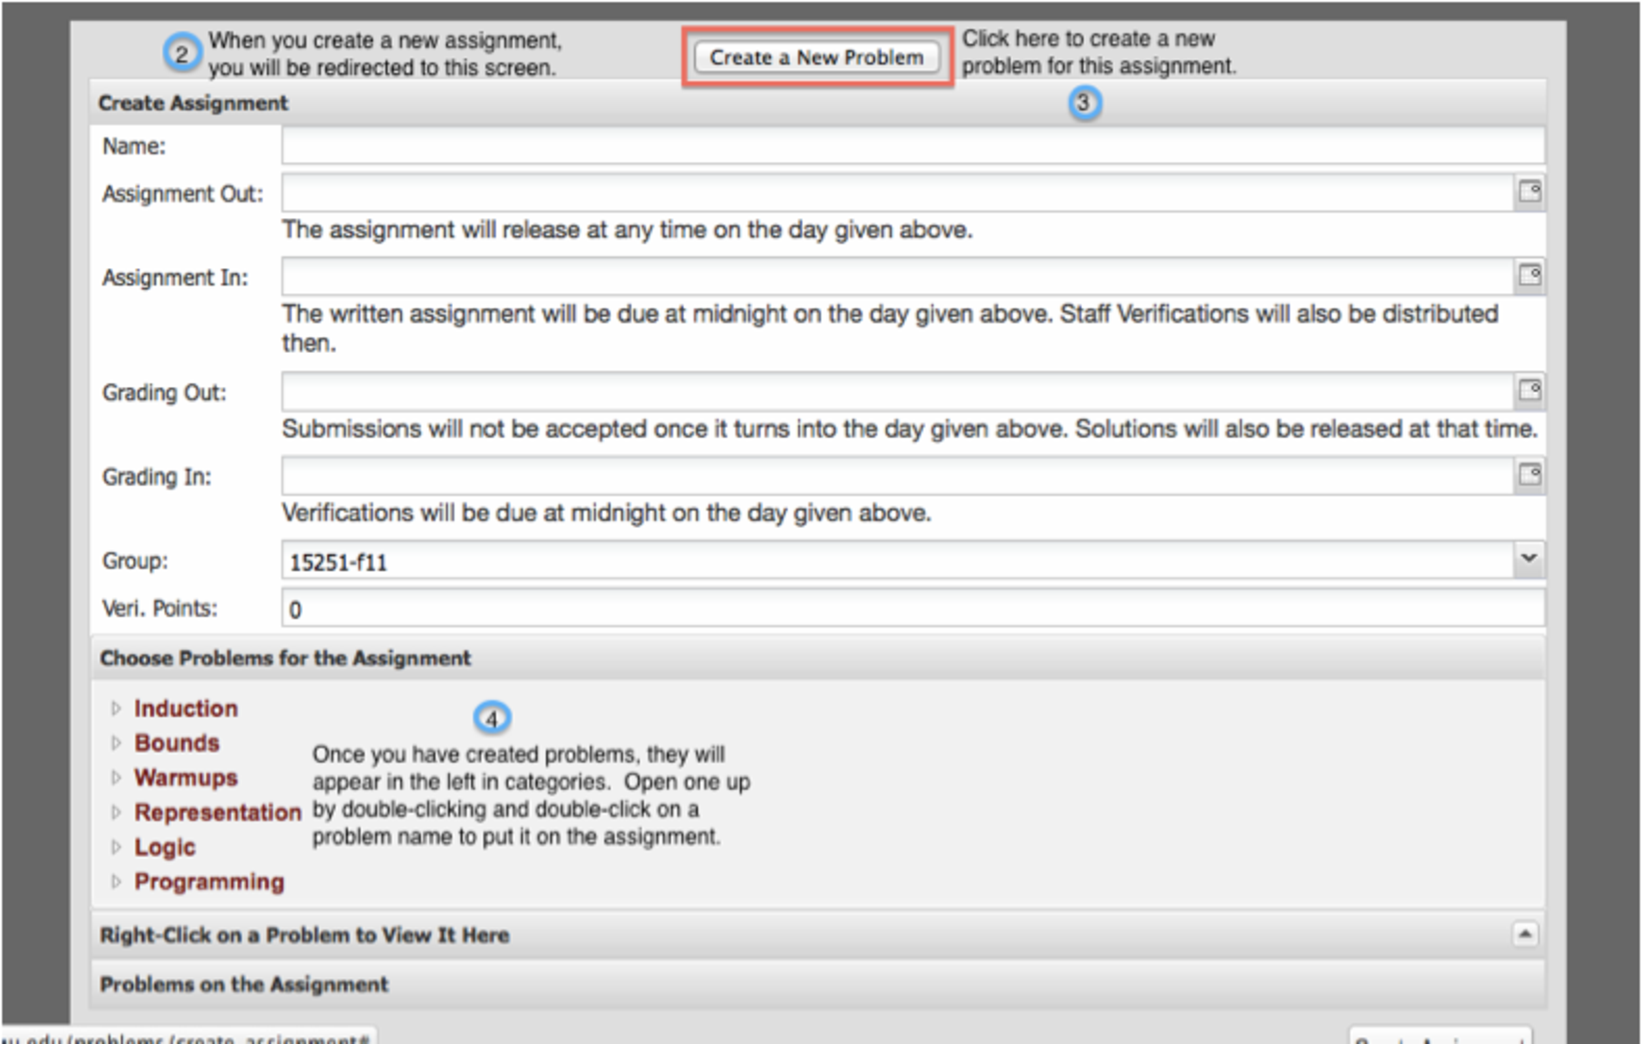
\includegraphics[scale=0.45]{screenshot-grading}
\end{center}
\caption{Screenshot of Prototype Proof Grading System}
\label{fig:screenshot}
\end{figure}

At Carnegie Mellon University, one of our undergraduate graders, Adam
Blank, created a system that serves as the prototype for the proposed
research.  Indeed, he is now a PhD student and this proposal seeks
funding to support him.  The system is designed to support large classes,
with the assessment performed by the students in the class and by
undergraduate graders.  It has been used in classes with enrollments
ranging from 60 to 380 students, in both computer science (introduction
to theoretical computer science) and mathematics (discrete math). 
Figure \ref{fig:screenshot} shows part of the interface of the system 
from the instructor's point of view.



Elements of this system demonstrate 
how a scalable and reliable peer assessment system can work.  First,
the task of assessing a proof is defined as one of identifying a set of
{\em attributes} that are applicable to a particular proof.  These are
positive and negative facts that may hold for the proof.  Example
attributes include:
\begin{itemize}
\item The proof is by induction on the size of the array.
\item The proof uses linearity of expectation.
\item The base case of the induction is correct.
\item The proof contains an arithmetic error.
\end{itemize}

The list of possible attributes for a problem is generated by the
instructor and by experienced graders, based on grading a sample of
around 15 proofs.  Of the 148 problems that have been graded with
attribute-based grading, nine had 100 or more applicable attributes,
while the average was 40.6.  

The actual grade for a proof is computed using a formula, devised
by the instructor, based on which attributes apply.  This mechanism
nearly eliminates any subjective evaluation by the less experienced graders
or the student reviewers and ensures uniformity of the grading
standards across the team of graders.  Each proof is reviewed by 3--5
students and by one grader.  The task for the student reviewers is to
identify which attributes they believe apply to a proof, while for the
grader it is to filter through the proposed attributes to see which
ones really do apply.  Having multiple reviews increases the chance
that the set of possible attributes will be complete.  To avoid
collusion, students are required to identify their collaborators,
forming edges in an undirected graph with students as nodes.  The
set of students is partitioned according to the connected components
of the graph, and
reviewers are assigned randomly, but such that they never review
assignments generated by students in their own components.

Reviewers are graded on the quality of their assessments, comparing
their results with those generated by the grader.  This is done with a
simple 0--2 point scale (0 = useless, 1 = somewhat helpful, and 2 =
accurate.)  These reviews comprise around 10\% of the course grade,
and so students are highly motivated to do a good job, although more
by coercion than by any perception of benefit on their part.

We can see how this prototype system implements a form of human computation,
enabling nonexperts to perform useful and reliable work.  The normally
subjective task of assessing a proof is put into a structured
framework, such that it can be decomposed into a number of simpler
tasks that can be performed by nonexperts.  Workers are assigned
different types of tasks according to their capabilities and trustworthiness.
Randomization, redundancy, and selectivity are used in the task assignment to
improve quality and to ensure integrity of the process.

Although the conditions for and scale of the deployment of our
prototype system were insufficient to perform a systematic evaluation,
we have gained some insights from anecdotal evidence and from a survey
conducted in one of the classes.  First, the system worked better than existing
rubric-based approaches.
The graders found that the student
reviewers generally identified all of the applicable attributes for a
proof, although their selections had to be pruned down and
occasionally augmented.  The graders found having this input from the
student reviewers useful, even though they still had to carefully
review the proofs themselves.  Second, the instructors found the
grades assigned to the proofs to generally be fair assessments of
their quality.  The idea of generating a score automatically from the
set of applicable attributes was seen as greatly improving the
uniformity of the grading, while also yielding appropriate scores.
Of course, we cannot claim these results without a more rigorous
evaluation, but they lend hope that the overall approach is viable.

A survey conducted of students in one class indicated that they had
mixed opinions about being required to participate in the reviewing
process.  The major complaint was that they were being asked to do
extra work in a course that was already perceived as requiring too much
work.  Even so, when asked whether they found performing the reviews
to be helpful to their understanding of the material, 42\% said yes,
28\% said no, and 30\% were neutral.  So, there is some justification
for claiming that having students perform peer reviews has an educational
value, but more must be done to maximize the real and perceived
educational benefit of doing reviews.

\subsection{Summary of Prior Work}

We see from this survey of prior work that our system stands out as
unique in providing a structured environment for students to review
each other's proofs in a systematic way.  This enables quality
assessment to be performed using the students themselves and a large
staff of undergraduate graders.  Nonetheless, our system is only a
prototype and requires much more work to solidify its design and to
evaluate its effectiveness.

\section{Coping with Scale}

Most large classes, including those using our prototype system, use a
two-level hierarchy for assessing student work.  A single instructor
guides the work of a staff of graders, who then oversee the efforts of
a much larger groups of students.  One simple model for such a system
is to assume that a single person can monitor the work of around $k$
others.  Then a two-level hierarchy can have one instructor running a
class with $k$ staff members and $k^2$ students.  A typical value
range for $k$ might be 20--40, making it possible to have classes with
enrollments ranging from 400 to 1,600.  Although this model is
obviously simplistic, we can see some validation with very large
courses.  For example, Prof.~James Maas of Cornell University was
renowned for teaching an introductory psychology course with 1,600
students, staffed by 22 teaching assistants \citep{arenson-nyt00}.
Harvard's introductory computer science course CS~50 has an enrollment
of around 600 students, and their web page lists over 50 staff
members.  In the former case, the graduate teaching assistants working
for Prof.~Maas could probably handle a heavier load than could the
undergraduates staffing the Harvard course.  We can also see more than
a simple two-level structure in the Harvard class, with some staff members
serving as teaching assistants and others as graders, but our
simplified model suffices for discussion purposes.

A two-level hierarchy suffices for almost any course at a single
institution, but it cannot grow to web scale, in that it would require
our factor $k$ to be 100 or more to staff a course with over 10,000
students.  One could institute a deeper hierarchy,
requiring $\log_k n$ levels of staffing for a course with $n$ students.
This would require a
total staff of around $n/(k-1)$ people.  For example, for $k = 30$, a
three-level hierarchy could handle 27,000 students, but it would
require over 900 staff members.  This would not be economically feasible
for a MOOC, where the intention is to offer the course at little or no
cost.  Instead, we must find ways to fill out the lower ranks of the
hierarchy using volunteer labor.  This can be done by identifying the
most capable students and providing them with incentives to help the
others.  In addition, it may be possible to recruit volunteers who
already know the material, perhaps by already having taken the course.
The challenge with this approach is then to devise a suitable
incentive system and to provide the necessary framework for the
volunteers, and the students themselves, to handle most of the load in
performing assessment.

\section{Proposed Work}

\begin{figure}
\begin{center}
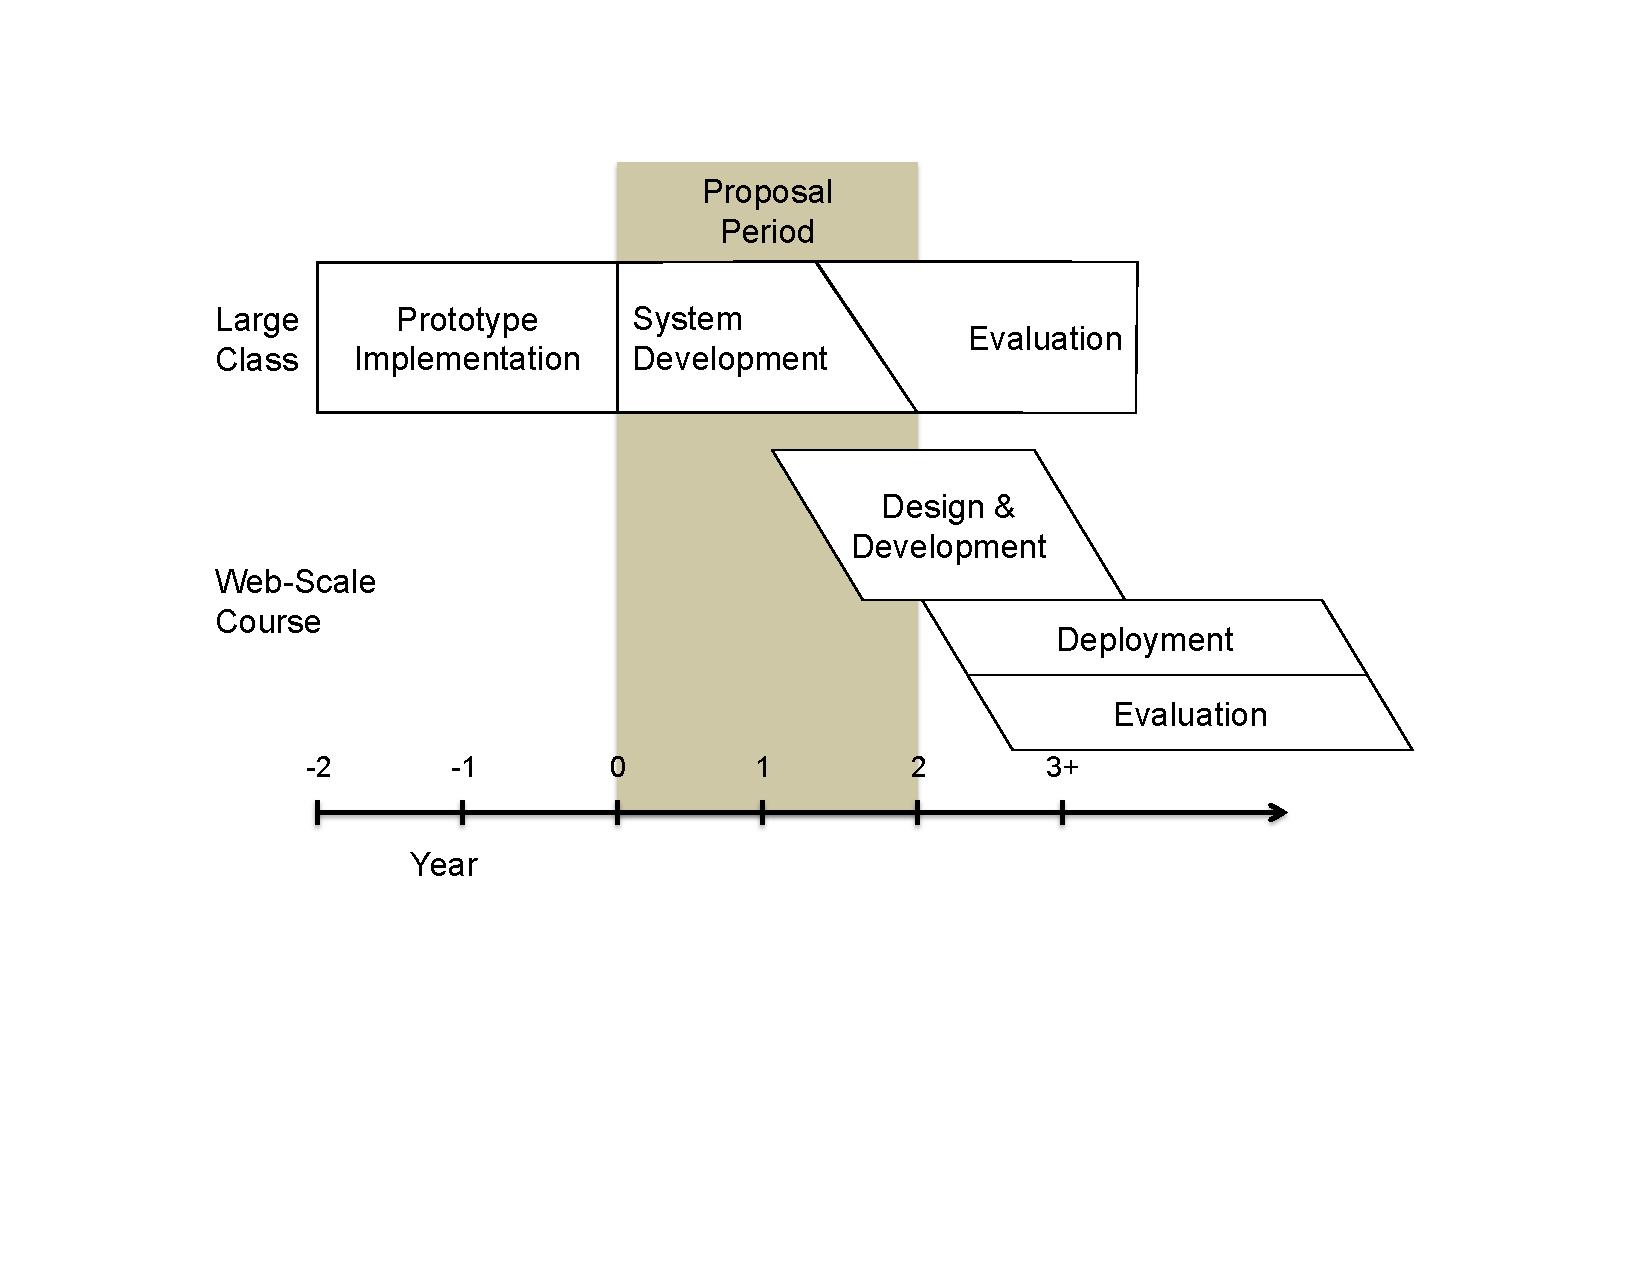
\includegraphics[scale=0.5]{schedule}
\end{center}
\caption{Proposed Activity Schedule}
\label{fig:schedule}
\end{figure}


Our long-term goal is to create educational technology that enables
students to learn how to write and evaluate proofs.  We propose
building on the ideas embodied in our prototype to support both large
classes and web-scale courses.  We will design our systems with the
twin objectives of maximizing the quality of the assessments produced, as
well as the learning value students gain by performing peer assessment.

Figure \ref{fig:schedule} illustrates how work over the two-year
period funded by this proposal fits into an overall plan.  (The
schedule shown in this figure is only approximate.)  As is indicated,
we have already invested two years of work in building and deploying
our prototype system.  During the proposal period, we will concentrate
mainly on supporting large classes using an improved system, including
the design, development, and deployment of an assessment system,
as well as initial steps in evaluating its
effectiveness.

Within the two-year period,
we will also begin work on a system to support
web-scale courses, but we anticipate that the majority of its design,
implementation, and deployment will take place after we
have gained more experience in large-class environments.  Once we have
this system in place, we will have many opportunities to evaluate its
effectiveness and to conduct quantitative experiments on how best to
teach students to write and evaluate mathematical proofs.

In the following we identify specific areas requiring further
attention and ideas for how they could be improved.  We also describe
possible evaluation approaches.

Just as with our prototype, we plan to deploy and evaluate
the technology within large computer science and
mathematics courses at Carnegie Mellon University.  This will give us
access to actual students and undergraduate graders in the context of
actual courses, all at no cost to the research project.

\subsection{Improving Assessment Quality}

Our first goal will be to create an assessment system that provides
reliable and accurate assessments in the context of a large,
undergraduate class.  It assumes that we have a staff of undergraduate
graders, ranging from those who have just taken the class to those who
have several semesters of grading experience and who have gained
mathematical maturity by taking more advanced courses.

Overall, the strategy of breaking the assessment of a proof down into a smaller
set of attributes seems effective, making the task manageable by
both student reviewers and graders, and also enabling a uniform
system for assigning scores.  In our current system, however, the set
of attributes is simply tabulated as a flat list.  We have found that
this lack of assessment structure fails to provide enough guidance to the
reviewers and the graders regarding how the different aspects of a
proof should fit together.

\subsubsection*{Pathway verification}

We would like to
create a more structured representation of proofs we call {\em pathway
  verification,}  where the required components of a proof are
explicitly identified.  Some example structures include:
\begin{itemize}
\item A proof by induction must contain an induction hypothesis,
  proofs of the base cases, and proofs of the induction steps.
\item The proof of an if-and-only-if property must have proofs of the
  ``if'' part and the ``only if'' part.
\item A case analysis must include proofs of each possible case.
\end{itemize}
In addition, more complex proofs should be broken down into a set of
lemmas with a valid dependency structure,
as can be captured by a proof graph \cite{anderson-science85}.

For problems assigned in the introductory and intermediate-level
courses we are targeting, there will only be a limited number of
possible pathway structures students can use.  These will be
determined by the instructional staff when devising the assignment and
by grading a sample of 15--25 proofs.  In doing their reviews, the
students will first identify the relevant pathway structure, and then
they will select attributes related to how successfully each component
of the pathway is covered in the proof.  The graders will then refine
the student reviews to devise the precise set of attributes.

We believe that the greater structure provided by pathways will
provide helpful guidance to the students and the graders when doing
their assessments.  It will also provide a useful tool for helping
students better understand how a proof should be structured.  One
could imagine, for example, assigning exercises where the
desired pathway for a proof is given, and the students must
then structure their proofs accordingly.

\subsubsection*{Assigning graders and reviewers}

Our current method of assigning proofs to reviewers attempts to avoid
conflicts of interest, but it is otherwise completely random.  We
believe we can achieve better results (both in terms of grading accuracy and learning outcomes) by making use of the
heterogeneity of the students, both as proof generators and reviewers,
and the grading staff.  In our experience, even at an elite
institution, there is a wide range of skill levels among the students.
Moreover, each student has different areas of relative strength and
weakness.  Similarly, the grading staff can range from those who took
the course in the previous semester to those who have served as
graders for several years.  In our experience, the graders get much
better at evaluating proofs over time.

In conventional settings, a common strategy in grading papers is to
first look at the ones from the top students to determine what the
best quality results are likely to be.  Similar strategies can be used
in a computer-mediated setting.  We can gain some idea of the likely
difficulty of assessing a proof from the prior history for this
student, as well as by some statistical analysis of the text.
Assuming Zerr's experience that correct proofs are much easier to
grade than incorrect ones, we can bias the assignment of reviewers and
graders so that the more challenging ones are assigned to the most
qualified assessors.

\subsubsection*{Providing Training on Assessment}

One way to improve the effectiveness of students performing peer
reviews would be to have them do explicit exercises for this task.
This could be done in a session where students are provided with a set
of proofs to assess that are known to represent a range of strategies,
including both valid and invalid examples.  They could then get
immediate feedback on the quality of their work, which is recognized
as an important principle for acquiring cognitive skills
\citep{anderson-jls95}.  Such training sessions could also serve as
opportunities to ``assess the assessors,'' so that we would have more
input to the process of assigning proofs to reviewers.


\subsubsection*{Evaluation}

There are multiple methods for measuring the effectiveness of an
assessment technique.  The most straightforward is to compare the
results to those generated by qualified assessors.  This can readily
be done by having an expert independently grade a set of
assignments, and then doing a comparison with the assessments
generated by our system.  In addition, we can evaluate the uniformity
of the assessment system by having multiple, independent assessments
of a single set of proofs.  Similar experiments can measure the
comparative effectiveness of different assessment systems.

Indeed, we claim that the baseline for the comparison
should not be that of an expert giving a careful review, but a more
typical setting where a group of 10 undergraduate graders is given 200
assignments to review.  If reviewing a proof requires 10 minutes, then
each grader must work for over three hours.  Our experience has been
that it is very difficult to maintain consistency across graders, and
even for the same grader over time.  We would like to quantify this
experience by conducting experiments that more closely model this
typical environment, and then see how much the structuring of the
assessment task and the presence of student
reviews accelerates the grading process and improves its quality.

\subsection{Improving Learning Experience}

Our prototype system compels students to provide peer reviews of each
other's proofs by making this an aspect of their course grade.
Ideally, however, we would
rather motivate students by having the review process serve as a useful
learning experience, both in truth and by their perception.

We believe that our adoption of a more structured representation of
proofs will enable the peer reviewers to better internalize the
appropriate proof structures.  They will get a detailed view of
alternate ways to prove something and to pinpoint places where a proof
is either invalid or incomplete.  Thus, our proposed work on pathway
verification will improve both the assessment quality and the learning
experience. 

Some aspects of the learning experience can also be optimized in the way
proofs are assigned to reviewers.  We want to assign to each student
a set of proofs that represents a diversity of possible solutions and
that is appropriate to his or her skill level.  In addition, we want
the assessment efforts to give the students a better understanding of
how a correct proof should be structured, and the likely ways in which
a proof can be invalid.
Based on the
prior history of the student writing the proof and by statistical
language analysis, we should be able to estimate properties, such as
1) whether the proof is likely to be correct, 2) how clear the presentation
will be, and 3) what pathway structure it follows.  Although this
information will not be completely reliable, we can use it to control
useful weights in the random process of assigning proofs to reviewers.

In maximizing the learning experience, we must take into account the
heterogeneity of the students, both in the quality of the proofs they
generate and their ability to review proofs.  Reviewers would learn
little by attempting to review proofs they cannot understand, nor
would such efforts generate useful assessments.  We therefore want to
assign each reviewer a set of proofs that will challenge him or her
intellectually, but at an appropriate level.

In some respects, there are fundamental tensions between the
objectives of 1) obtaining accurate assessments, 2) maximizing the
learning value, and 3) making the review process enjoyable (or at
least less onerous.)  For example, one way to maximize assessment
accuracy would be to increase the level of specialization among
reviewers.  One reviewer might be better at assessing a particular
style of proof or might be especially good at identifying the flaws in
a proof.  Such specialization, however, would not give the reviewers
the chance to develop a broad set of skills.  Furthermore, a reviewer
would find it monotonous to only review one class of proofs.
Similarly, we do not want to ``punish'' the best students by making
them always review the most flawed proofs.

One way to overcome this tension is to increase the level of
redundancy in assigning proofs to reviewers, beyond that required to
ensure assessment quality.  For example, we could ensure that everyone
gets a chance to study a high quality proof by increasing the number
of reviews for an exemplary proof.  Such proofs could be identified by
the graders or other reviewers, or they could even be crafted by the
staff.  Similarly, we might want to seed the reviewing process with
proofs that are known to contain flaws, so that students get
practice identifying specific classes of errors.  Similar strategies
would allow us to fine tune the range of proof types and proof
qualities that the students review.

Evaluating the students' perception of the learning benefit of
performing peer reviews can readily be done via surveys.  Evaluating
the actual learning benefit is more difficult, but we can gain some
insight by running A/B experiments across different sections of a
single course, or across the different offerings of a course over time
\citep{kohavi-dmkd09}.  However, the value of such experiments is
limited by the many experimental factors that cannot be controlled,
and by the small sample size of a course within a single institution.
We believe that this aspect of the assessment system will best be
evaluated when we move to web-scale courses.  As will be discussed,
such an environment provides more opportunities to run reliable
quantitative experiments of learning effectiveness.

\subsection{Scaling to Web-Scale Courses}

Within the two-year period covered by this proposal, we can only
begin our efforts to support web-scale courses, as shown in Figure
\ref{fig:schedule}.  We present some preliminary ideas on the
challenges and opportunities of working at this scale, since our
intention is to continue past the proposal period with a more
ambitious range of activities.

As we have discussed, a true web-scale course cannot rely on a
two-level hierarchy.  Indeed, if the course is to be offered at little
or no cost, the instructor can only have a small set of assistants.
We therefore cannot have paid staff directly oversee the efforts of
individual students, as we did with large classes.  We must therefore
find a method to recruit volunteer labor, including current and former
students from the course.  In addition to providing incentives to
motivate these volunteers, we must have a very structured and reliable
framework that will ensure that the assessments are of high quality.
Fortunately, systems such as Wikipedia demonstrate that skilled labor
can be recruited to do useful work for free, when provided proper incentives
\citep{nov-cacm07}.

Some aspects of web-scale courses simplify the assessment task.
Given that current and planned MOOCs do not provide
any form of authenticated credential, the purpose of assessment in
these courses is more to help the student (formative) rather than to
measure performance (summative).  There is therefore less need for
uniformity and reliability of the assessment and for preventing
collusion among the students and between students and assessors.

We believe that our system for supporting assessments of proofs in
large classes can be scaled to handle web-scale classes.  Typically,
the web-scale course will be based on one that has already been
taught using our system, and so a sufficient set of possible attributes and
pathway structures will already have been generated.  The role of the
instructor and staff will be very different than is the case for a
large class.  They will set up the assessment framework and oversee
its operation, but they will not do any of the assessment themselves,
beyond a small initial sample and perhaps some exceptional cases.

As with a large class, we will get all of the students in the course
to perform reviews of each other's proofs.  Rather than using paid
staff to condense the peer reviews into a final assessment, we will
use a specially qualified group of ``super reviewers,'' working on a
volunteer basis.  As mentioned earlier, these could be current or
former students whom we identify as having sufficient talent to
perform this task.

We could provide various incentives for qualified people to serve as
super reviewers, according to how the MOOC supports itself and how it
motivates the students to participate.  For example, we could set up a
rating system where the super reviewers get public recognition for
their efforts.  For a MOOC that receives revenue from potential
employers by identifying its top students to them, we could also
direct the top super reviewers to them.  We could reward the top super
reviewers by inviting them to special events, as is done with the top
Wikipedians.  Indeed, the super reviewers could fill out much of the
hierarchy in the course operation, with the top ones performing such
tasks as generating new attributes or pathway structures for a proof,
or even devising new assignments.

\section{Long Term Plans}

Looking further into the future, we see many opportunities to build on
the proof assessment systems we will develop for large classes and for
web-scale courses.

\subsection{Web-Scale Courses as Experimental Learning Platforms}

In addition to providing a valuable service to society, web-scale
courses have the potential to serve as rich platforms for experimental
research in learning science.  In the case of proof assessment,
operating at a web scale will allow us to rigorously evaluate the
effectiveness of the system, and indeed to gain much deeper insight
into the most effective methods to teach students how to write and
evaluate mathematical proofs.

The large number of participants in a web-scale course provide a more
reliable statistical sample than is possible in any classroom
environment.  Moreover, the students are less likely to interact with
one another outside of the experimental environment, and so there will
be less tainting of control groups or between participants in A/B
testing.  Furthermore, we can conduct experiments at very fine levels
of granularity, where only small variations in conditions are
evaluated among the different populations.  The fact that MOOCs are
very inexpensive (typically free), and that they do not supply an
authenticated credential reduces the ethical concerns regarding whether
some students receive suboptimal learning experiences.

As an example, a web-scale course will enable us to truly evaluate the
learning value students obtained by participating in peer reviews.  We
can run experiments where one group does no peer reviewing and another
does, and then evaluate student achievement across the two groups.  By
contrast, such an experiment does not work as well in a single
traditional class, because the students soon realize that they
are being asked to participate in different tasks, leading to a
tainting of the experiment.  Attempting to run such an experiment
across multiple traditional classes, either temporally or at different
institutions has the same risk of tainting, while also being difficult
to achieve statistical uniformity across the two populations in other
respects.

Beyond answering large questions, such as ``Does participating in peer
reviewing make students learn the material better?'' our platform can
allow us to test the effectiveness of more incremental changes, such
as how proofs are assigned to reviewers, what framework is provided
for the review process, etc.  Since the student experience can be
controlled in very detailed and individualized ways, and all of the
data will be collected in electronic form, we will have experimental
capabilities far beyond what is possible in a conventional learning
environment.

\subsection{Additional Deployments}

Our proof assessment system will be useful for a range of courses in
mathematics and computer science.  It is especially appropriate for
beginning and intermediate-level courses, where the range of possible
proofs for a problem is limited, and where the focus is more on proof
correctness, rather than quality of exposition.

We will actively seek partners at other institutions to make use of
our system.  The system will work, however, only if many students take
a course at the same time, so that we can get a large enough pool of
reviewers, while minimizing the chances of collusion.  This requires
either targeting large-enrollment classes, or using it for a course
that is taught (identically) across multiple institutions.  Of course,
it also requires an instructor who is motivated to try
out a new and relatively untested system.

\subsection{Beyond grading proofs}

Our assessment system focuses on mathematical proofs, but we believe
there are other review activities for which similar, peer-based assessment
could be applied.  What we require are activities that cannot
be fully automated, but there is enough structure to the process that
the work can be decomposed into simple tasks that can be performed by
nonexperts.  In addition, we would hope that participating in the review
process would help them improve their own skills.

Some examples of suitable review activities include:
\begin{itemize}
\item
Evaluation of programs for style, based on conformance to a set of
coding guidelines.  This can be divided into such tasks as assessing
the suitability of variable and function names, the quality of the
commenting, and the use of modularity.  Indeed, a system along these
lines is under development at MIT and has already been used by around 400
students \citep{tang-mit11}.

\item
Code review for specific properties, such as security vulnerabilities,
memory management errors, or efficiency.

\item
Low-level text editing, such as for written assignments in an ESL course.
\end{itemize}

As these examples show, we believe that human computation can
compensate for the lack of direct human contact in a variety of
large-scale learning environments.  In doing so, we can make high
quality education available to large groups of people at very low
cost.  Such tools also provide opportunities to run rigorous and
detailed experiments on the effectiveness of teaching strategies, with
the possibility that we can become more effective at education using
online tools than is possible with conventional approaches.

\section{Results from Prior NSF Support}

Of the two PIs, only Luis von Ahn has received NSF support within the
last five years. 

Luis von Ahn is senior personnel of the NSF grant ``Collaborative 
Research: HCC: Large: Design Principles for Information Networks, 
Supporting the Social Production of Knowledge,'' (PI Jon Kleinberg, 
NSF award number IIS-0910453 for \$2,061,727, awarded from July 15, 
2009 to June 30, 2014), which supports research in social networks, 
specifically the effects of ``network shaping'' on the behavior of the 
users, and it is largely unrelated to the current proposal.

Luis von Ahn is a PI of the NSF grant ``SoCS: Effectively Leveraging 
Contributors in Human Computation Systems'' (co-PI Tom Mitchell, NSF 
award number IIS-0968487 for \$737,500), which aims to better 
understand how each individual's different capabilities in a human 
computation system can be assessed and dynamically leveraged. This 
grant has provided improved understanding of the strengths and weaknesses 
of human users as teachers and data sources for machine learning 
algorithms, and an intelligent new objective-driven model of data 
collection. It has supported the following publications:

\begin{itemize}

\item E. Law and B. Settles and A. Snook and H. Surana and L. von 
Ahn and T. Mitchell.  ``Human Computation for Attribute and 
Attribute Value Acquisition.'' {\em CVPR Workshop on Fine-Grained 
Visual Categorization}, 2011.

\item E. Law, B. Settles and T. Mitchell.  ``Learning to Tag From Open 
Vocabulary Labels.'' {\em ECML 2010}.

\item H. Zhang, E. Law, R. Miller, K. Gajos, D. Parkes, E. Horvitz.  
``Human Computation with Global Constraints: A Case Study.''  In 
{\em CHI, 2012}.

\item E. Law and H. Zhang. ``Towards Large-Scale Collaborative 
Planning: Answering High-Level Search Queries using Human 
Computation.'' {\em AAAI, 2011}.
\end{itemize}

Finally, Luis von Ahn is the PI for the NSF grant ``CAREER: Online 
Education as a Vehicle for Human Computation'' (NSF award number 
1054630), whose central hypothesis is that problems that are difficult 
for computers can be transformed into tasks that are also educational, 
so that students solve the problems at the same time as they learn.
This grant has supported the development of http://duolingo.com, which
will be released to the public on June 19, 2012.

\newpage
\setcounter{page}{1}

\bibliography{refs}

\end{document}
